\documentclass[12pt,letterpaper]{article}
\usepackage{graphicx,textcomp}
\usepackage{natbib}
\usepackage{setspace}
\usepackage{fullpage}
\usepackage{color}
\usepackage[reqno]{amsmath}
\usepackage{amsthm}
\usepackage{fancyvrb}
\usepackage{amssymb,enumerate}
\usepackage[all]{xy}
\usepackage{endnotes}
\usepackage{lscape}
\newtheorem{com}{Comment}
\usepackage{float}
\usepackage{hyperref}
\newtheorem{lem} {Lemma}
\newtheorem{prop}{Proposition}
\newtheorem{thm}{Theorem}
\newtheorem{defn}{Definition}
\newtheorem{cor}{Corollary}
\newtheorem{obs}{Observation}
\usepackage[compact]{titlesec}
\usepackage{dcolumn}
\usepackage{tikz}
\usetikzlibrary{arrows}
\usepackage{multirow}
\usepackage{xcolor}
\newcolumntype{.}{D{.}{.}{-1}}
\newcolumntype{d}[1]{D{.}{.}{#1}}
\definecolor{light-gray}{gray}{0.65}
\usepackage{url}
\usepackage{listings}
\usepackage{color}

\definecolor{codegreen}{rgb}{0,0.6,0}
\definecolor{codegray}{rgb}{0.5,0.5,0.5}
\definecolor{codepurple}{rgb}{0.58,0,0.82}
\definecolor{backcolour}{rgb}{0.95,0.95,0.92}

\lstdefinestyle{mystyle}{
	backgroundcolor=\color{backcolour},   
	commentstyle=\color{codegreen},
	keywordstyle=\color{magenta},
	numberstyle=\tiny\color{codegray},
	stringstyle=\color{codepurple},
	basicstyle=\footnotesize,
	breakatwhitespace=false,         
	breaklines=true,                 
	captionpos=b,                    
	keepspaces=true,                 
	numbers=left,                    
	numbersep=5pt,                  
	showspaces=false,                
	showstringspaces=false,
	showtabs=false,                  
	tabsize=2
}
\lstset{style=mystyle}
\newcommand{\Sref}[1]{Section~\ref{#1}}
\newtheorem{hyp}{Hypothesis}

\title{Problem Set 2}
\date{Due: October 22, 2026}
\author{William Sarsfield}

\begin{document}
	\maketitle
	\section*{Instructions}
\begin{itemize}
	\item Please show your work! You may lose points by simply writing in the answer. If the problem requires you to execute commands in \texttt{R}, please include the code you used to get your answers. Please also include the \texttt{.R} file that contains your code. If you are not sure if work needs to be shown for a particular problem, please ask.
	\item Your homework should be submitted electronically on GitHub.
	\item This problem set is due before 23:59 on Thursday October 22, 2026. No late assignments will be accepted.

\end{itemize}

	
	\vspace{.5cm}
	\section*{Question 1: Political Science}
		\vspace{.25cm}
	The following table was created using the data from a study run in a major Latin American city.\footnote{Fried, Lagunes, and Venkataramani (2010). ``Corruption and Inequality at the Crossroad: A Multimethod Study of Bribery and Discrimination in Latin America. \textit{Latin American Research Review}. 45 (1): 76-97.} As part of the experimental treatment in the study, one employee of the research team was chosen to make illegal left turns across traffic to draw the attention of the police officers on shift. Two employee drivers were upper class, two were lower class drivers, and the identity of the driver was randomly assigned per encounter. The researchers were interested in whether officers were more or less likely to solicit a bribe from drivers depending on their class (officers use phrases like, ``We can solve this the easy way'' to draw a bribe). The table below shows the resulting data.

\newpage
\begin{table}[h!]
	\centering
	\begin{tabular}{l | c c c }
		& Not Stopped & Bribe requested & Stopped/given warning \\
		\\[-1.8ex] 
		\hline \\[-1.8ex]
		Upper class & 14 & 6 & 7 \\
		Lower class & 7 & 7 & 1 \\
		\hline
	\end{tabular}
\end{table}

\begin{enumerate}
	
	\item [(a)]
	Calculate the $\chi^2$ test statistic by hand/manually (even better if you can do "by hand" in \texttt{R}).\\
		\lstinputlisting[language=R, firstline=2, lastline=20]{PS02_answersWS.R}  
		\begin{verbatim}
			The X^2 statistic is: 3.791168
		\end{verbatim}
	\vspace{7cm}
	\item [(b)]
	Now calculate the p-value from the test statistic you just created (in \texttt{R}).\footnote{Remember frequency should be $>$ 5 for all cells, but let's calculate the p-value here anyway.}  What do you conclude if $\alpha = 0.1$?\\
		\lstinputlisting[language=R, firstline=23, lastline=26]{PS02_answersWS.R}  
		\begin{verbatim}
		The p-value from the test stat is: 0.1502306
	\end{verbatim}
	With the p-value gathered from the test stat I can see that the p-value is .1502306 which is greater than .1 at the 90 percent confidence level. Therefore the conclusion that I reach is that I fail to reject the null of independence and that whether people are stopped by police officers is not dependent on class.
	\newpage
	\item [(c)] Calculate the standardized residuals for each cell and put them in the table below.
	\vspace{1cm}
	
	\begin{table}[h]
		\centering
		\begin{tabular}{l | c c c }
			& Not Stopped & Bribe requested & Stopped/given warning \\
			\\[-1.8ex] 
			\hline \\[-1.8ex]
			Upper class  & 0.3220306 & -1.641957  & 1.523026  \\
			\\
			Lower class & -0.3220306  & 1.641957  & -1.523026   \\
			
		\end{tabular}
	\end{table}
		\lstinputlisting[language=R, firstline=29, lastline=42]{PS02_answersWS.R}  
	
	\vspace{1cm}
	\item [(d)] How might the standardized residuals help you interpret the results?  
	\vspace{1cm}
	\noindent
	
	 The standardized residuals help us interpret how far away each observation is from the predicted or expected value. The denominator shows how many standard errors the observation is from the expected value. This statistic helps me interpret the observations as it demonstrates that upperclass not stopped, upper class and stopped/given warning as well as lower class and bribe requests all had more observations than expected.  While on the other end the lower class and not stopped, bribe requested and upper class, and lower class and stopped/given warning all had a lower number of observations in this study than expected.
	
	 It is also noteworthy that all the standardized residuals sum to zero in the total table as well as in each column. 
	 
\end{enumerate}
\newpage

\section*{Question 2: Economics}
Chattopadhyay and Duflo were interested in whether women promote different policies than men.\footnote{Chattopadhyay and Duflo. (2004). ``Women as Policy Makers: Evidence from a Randomized Policy Experiment in India. \textit{Econometrica}. 72 (5), 1409-1443.} Answering this question with observational data is pretty difficult due to potential confounding problems (e.g. the districts that choose female politicians are likely to systematically differ in other aspects too). Hence, they exploit a randomized policy experiment in India, where since the mid-1990s, $\frac{1}{3}$ of village council heads have been randomly reserved for women. A subset of the data from West Bengal can be found at the following link: \url{https://raw.githubusercontent.com/kosukeimai/qss/master/PREDICTION/women.csv}\\

\noindent Each observation in the data set represents a village and there are two villages associated with one GP (i.e. a level of government is called "GP"). Figure~\ref{fig:women_desc} below shows the names and descriptions of the variables in the dataset. The authors hypothesize that female politicians are more likely to support policies female voters want. Researchers found that more women complain about the quality of drinking water than men. You need to estimate the effect of the reservation policy on the number of new or repaired drinking water facilities in the villages.
\vspace{.5cm}
\begin{figure}[h!]
	\caption{\footnotesize{Names and description of variables from Chattopadhyay and Duflo (2004).}}
	\vspace{.5cm}
	\centering
	\label{fig:women_desc}
	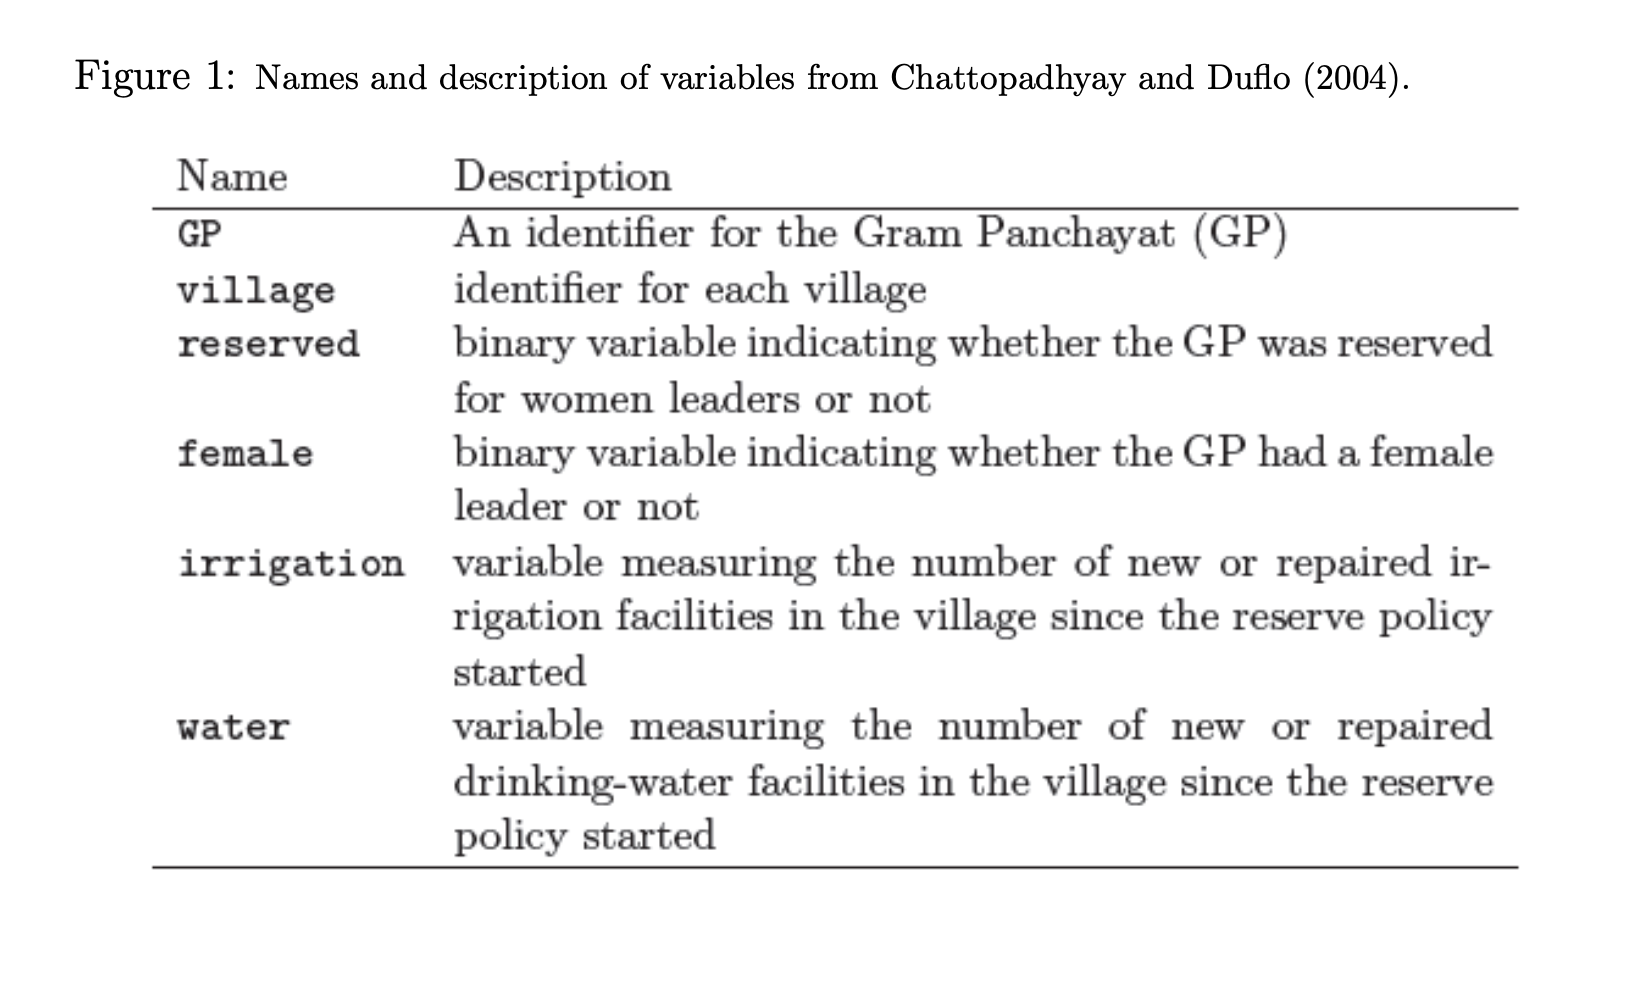
\includegraphics[width=.75\textwidth]{Imagine.png}
\end{figure}		

\newpage
\begin{enumerate}
	\item [(a)] State a null and alternative (two-tailed) hypothesis. 
\noindent


Ho: beta1 = 0 vs Ha : beta1 != 0


Ho: There is no relationship between reservation policy and the number of new or repaired drinking water facilities in the villages.


Ha: There is a relationship between reservation policy and the number of new or repaired drinking water facilities in the villages.
	\noindent 
	\vspace{6cm}
	\item [(b)] Run a bivariate regression to test this hypothesis in \texttt{R} (include your code!).
	\lstinputlisting[language=R, firstline=44, lastline=70]{PS02_answersWS.R} 
		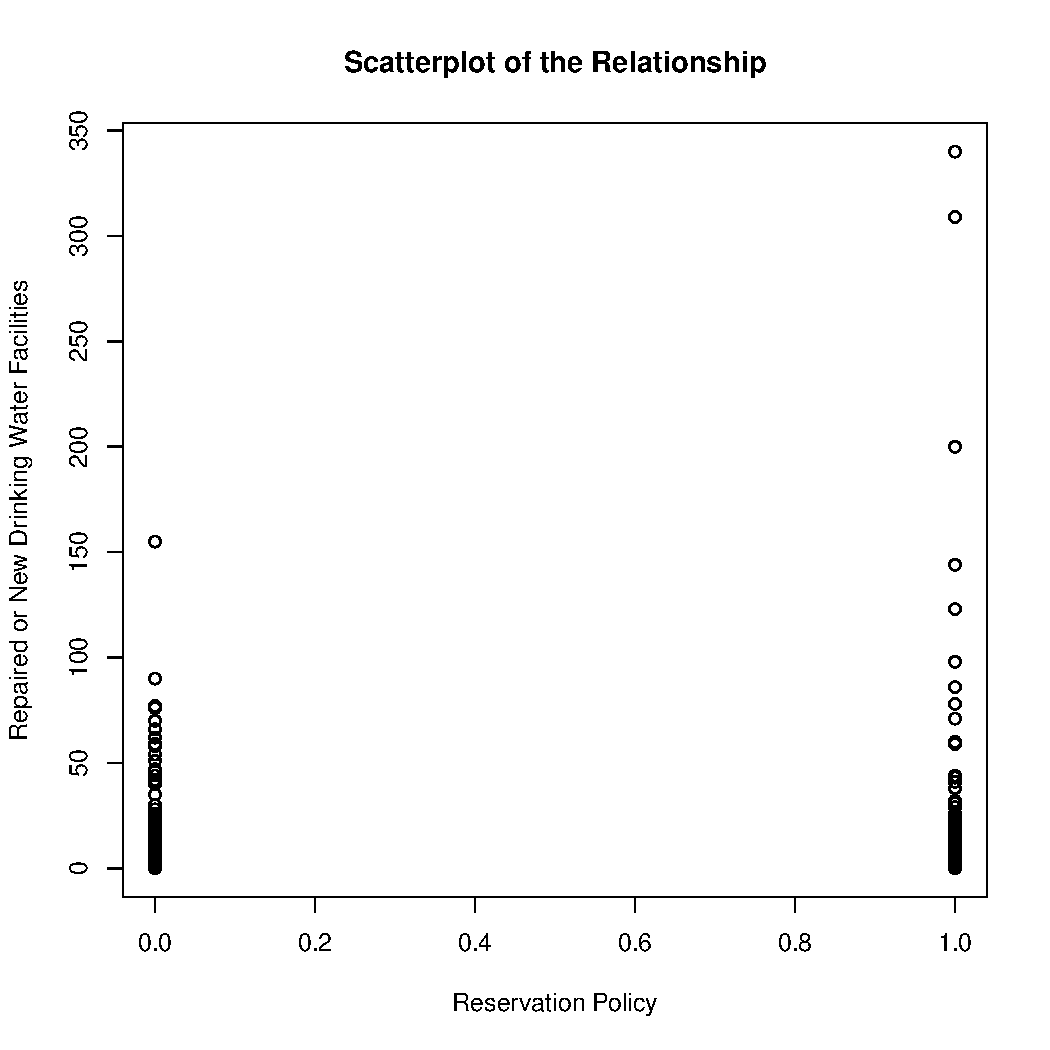
\includegraphics[width=.75\textwidth]{FirstPlot.pdf}
		\vspace{5cm}
	
	
		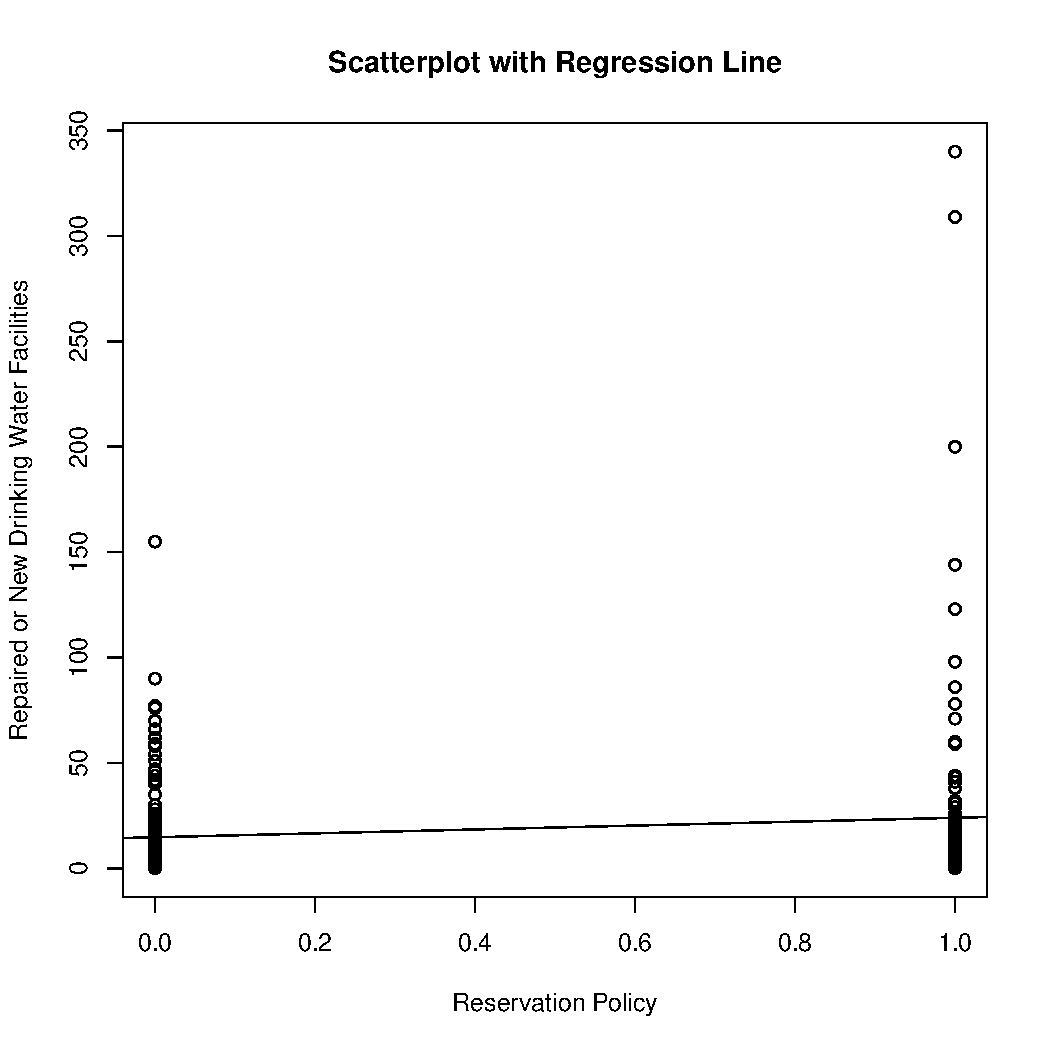
\includegraphics[width=.75\textwidth]{SecondPlot.pdf}
		\begin{verbatim}
		the correlation coefficient is found to be: 0.1299079 
		the correlations p-value is: 0.0197 
		allowing me to reject the null that reservation policy and 
		repaired or new drinking water facilities are not correlated
	\end{verbatim}
	\lstinputlisting[language=R, firstline=71, lastline=78]{PS02_answersWS.R} 
		\begin{verbatim}
		Manually I found the slope and the intercept. The slope is: 9.252423 
		and the intercept is: 14.73832
	\end{verbatim}
	\lstinputlisting[language=R, firstline=79, lastline=81]{PS02_answersWS.R} 
	\begin{verbatim}
		sd estimate is: 33.44568 double checked with sigma(model) which got 33.44568
	\end{verbatim}
		\lstinputlisting[language=R, firstline=82, lastline=89]{PS02_answersWS.R} 
	\begin{verbatim}
			Manually I found the pvalue for the slope and the intercept 
			the B1 p-value is: 0.01970398 
			and the B0 or alpha's p-value is: 4.216474e-10
\end{verbatim} 
			\lstinputlisting[language=R, firstline=90, lastline=97]{PS02_answersWS.R} 
	\begin{verbatim}
		The confidence interval for the slope is: 2.740105 15.76474
	\end{verbatim}
	\lstinputlisting[language=R, firstline=98, lastline=101]{PS02_answersWS.R} 
		\begin{verbatim}
	The amount of variability in repaired or new drinking water 
	facilities explained by reservation policy is: 0.01687605 
	or better stated as 1.7%
	\end{verbatim}
	\vspace{2cm}
	\item [(c)] Interpret the coefficient estimate for reservation policy. 
	\vspace{1cm}
	\noindent 
	
Using the coefficient estimate for reservation policy, which means that on average when a GP seat was reserved for women leaders the amount of new or repaired drinking water facilities in the village since the reservation policy started increased on average by 9.25.
Further, the slope was statistically significant and 0 was outside the constructed confidence interval allowing me to reject the null hypothesis that reservation policy does not help predict the number of new or repaired drinking water facilities. Overall reservation policy provides significant help in predicting the increase in drinking water facilities. The only issue with this remains the fact that this study tests a binary variable. Which means the coefficient for the slope of this line can only tell the difference between no reservation policy and reservation policy nothing in between and nothing further. Also this slope cannot be extrapolated for further values which would be bad practice still even with a more continuous explanatory variable. Lastly, this variable can not  tell how an increase in the number of reserved seats could impact the number of new or repaired drinking water facilities. 


Further the low amount of variability of drinking water facilities explained by reservation policy, which means there could be other more notable effects on the drinking water facilities being built and repaired than just reservation policy. 


\end{enumerate}


%\end{enumerate}
\end{document}
